\section{Ausblick}
Die aktuellste Version, also 1.2., wurde 2008 veröffentlich. In Bezug auf den Fortschritt im Hardware- und Softwarebereich gilt eine Technologie die mehrere Jahre zurück liegt schon als veraltet. Dahin gehend wurde eine Roadmap entwickelt, die aktuelle Neuerungen im Bereich HTML5, CSS3 und CSS4, Webschnittstellen und verschiedene Medien direkt einbinden kann. Diese neue Iteration soll dann als SVG 2.0 veröffentlicht werden. In der Abbildung \ref{roadmap} sieht man einen Zeitstrahl zur Roadmap. Im folgenden kann nur eine ungefähre Angabe über die Neuerungen erfolgen, da die Entwicklung der Recommendation noch in den Anfängen steht.\\

\begin{figure}[!ht]
  \centering
  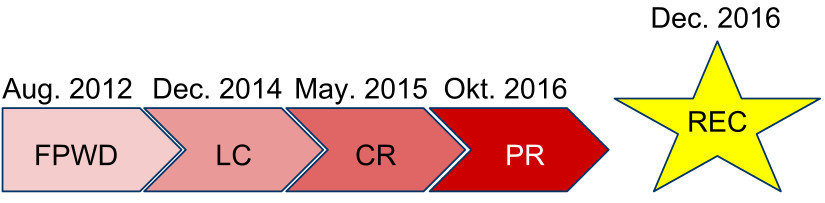
\includegraphics[width=0.95\textwidth]{pictures/roadmap.jpg}
  \caption{Roadmap zur Recommendation SVG 2.0. FPWD : First Public Working Draft,
    LC : List of Candidates,
    CR: Candidatest Recommendation,
  PR: Proposed Recommendation}
  \label{roadmap}
\end{figure}
Eine Neuerung wird sein, dass mehr CSS3 und CSS4 Befehle direkt als Attribute eingebunden werden können. Diese Attribute konnten bislang, wie bei HTML Tags üblich, auch schon über das "style"-Attribut benutzt werden. Um eine bessere Übersicht über die Möglichkeiten innerhalb eines Standards zu ermöglichen, wurde sich entschieden, die Attribute zu erweitern.\\
Zum Beispiel wird das "textoverflow" Attribut integriert. Hierbei kann der Programmierer selbst bestimmen, was mit Textbausteinen passiert, die voluminöser sind, als das vorgegebene Element. Dabei kann entschieden werden, ob diese einfach unberührt ausgeschrieben oder abgekürzt werden oder im Baustein verschwinden. \todo{Quelle}\\
Ein weiteres Beispiel ist das Farbkonzept, dass manigfaltiger im neuen Standard integriert wird. Darunter fällt nicht nur, dass mehr Farbbezeichnungen benutzt werden können, sondern auch dass der Programmierer bestimmen kann, in welchem Farbraum die Farbe kodiert und eingegeben wird.\\

Eine weitere Neuerung wird vermutlich die Integration von medialen Inhalten sein, wie Bilder, Audios, Videos, iFrames oder Canvas. Wie weiter oben erwähnt kann unter bestimmten Umständen das Canvas performanter werden. Die ganzen Elemente werden unter dem Begriff Embedded Content zusammengefasst.\\
\todo{mehr Ausblick möglich, nur bin ich schon über das Limit drüber}

